\section{Preliminary Definitions}
\label{sec:background}

\subsection{Domain-Specific Languages in a nutshell}

%As aforementioned, a DSL is a set of language constructs each of which represents certain abstraction in a particular domain. In the general case, a DSL offers an editor that provides the capabilities needed to write programs (textually or graphically) by using the language constructs. Once a the program is written, it can be used as part of the implementation artifacts of a system under construction. 

\subsubsection{Specification:} Like general purpose languages (GPLs), DSLs should be defined in terms of syntax and semantics \cite{Harel:2004b}. Hence, the specification of a DSL is a tuple $<syn,sem>$ where $syn$ (the \textit{\textbf{syn}tax}) refers to the structure of the DSL and specifies each language construct in terms of its name and the relationships it has with other language constructs. In turn, $sem$ (the \textit{\textbf{sem}antics}) refers to the meaning of the language constructs. This meaning corresponds to the dynamic behavior of each language construct and defines the manner in which they are manipulated at runtime.

%The \textit{concrete syntax} refers to the association of the language constructs to the set of symbols (either graphical or textual) offered by the editor.
\vspace{-3mm}
\subsubsection{Technological space:} Currently, there are diverse techniques available for the implementation of syntax and semantics of DSLs \cite{Mernik:2005b}. Language designers can choose between using context-free grammars or metamodels as specification formalism for syntax. Similarly, there are at least three methods for expressing semantics: operationally, denotationally, and axiomatically \cite{Mosses:2001}. In this paper we are interested on DSLs which syntax is specified by means of metamodels and semantics is specified operationally as a set methods (a.k.a, \textit{domain-specific actions} \cite{Combemale:2013}). Each language construct is specified by means a metaclass and the relationship between language constructs are specified as references between metaclasses. In turn, each metaclass contains a set of domain-specific actions that correspond to the behavior at runtime.

\vspace{-3mm}
\subsubsection{Implementation:} In order to implement a DSL, language designer need a set of tools offering the capabilities to specify the DSL according to the selected technological space. Those tools are provided by language workbenches that offer a set of meta-languages for expressing syntax and semantics. The ideas presented in this paper are implemented in an Eclipse-based language workbench. In particular, metamodels are specified in the Ecore language whereas domain-specific actions are specified as methods in Xtend programming language\footnote{\url{http://www.eclipse.org/xtend/}}. The mapping between metaclasses and domain-specific actions is specified by using the notion of aspect introduced by the Kermeta 3 and Melange as explained in \cite{degueule:2015}. 

\subsection{On the notions of \textit{commonalities} and \textit{potential reuse} in DSLs}

By definition, DSLs are scoped to specific domains so they provide restricted set of language constructs. As a result, there is a proliferation of many DSLs in the literature each of which is useful in certain application contexts \cite{Mernik:2005b}. Although many of those existing DSLs are completely different and tackle independent domains; there are related DSLs with overlapping domains \cite[p. 60-61]{voelter:2013}. That is, they share certain language constructs i.e., they have \textbf{commonalities} between them. If two DSLs have commonalities and they are specified in the same technological space, then there is \textbf{potential reuse} since the specification of those shared constructs can be specified once and reused in the two DSLs \cite[p. 60-61]{voelter:2013}.

Naturally, commonalities can be found not only at the level of the syntax but also at the level of the semantics. For the technological space discussed in this paper, syntactic commonalities appear where DSLs share some metaclasses and semantic commonalities appear where DSLs share some domain-specific actions. Figure \ref{fig:domains} illustrates this situation. There are three DSLs (i.e., $A$, $B$, and $C$) with both syntactic and semantic commonalities. Syntactic commonalities (at the left of the figure) correspond to the metaclasses $MC_Z$ and $MC_Q$. $MC_Z$ is shared by DSLs $A$ and $C$ whereas $MC_Q$ is shared by DSLs $A$, $B$, and $C$. Semantic commonalities (at the right of the figure) correspond to the domain-specific action $DSA_3$ which is shared by all the DSLs. 

\begin{figure}
\centering
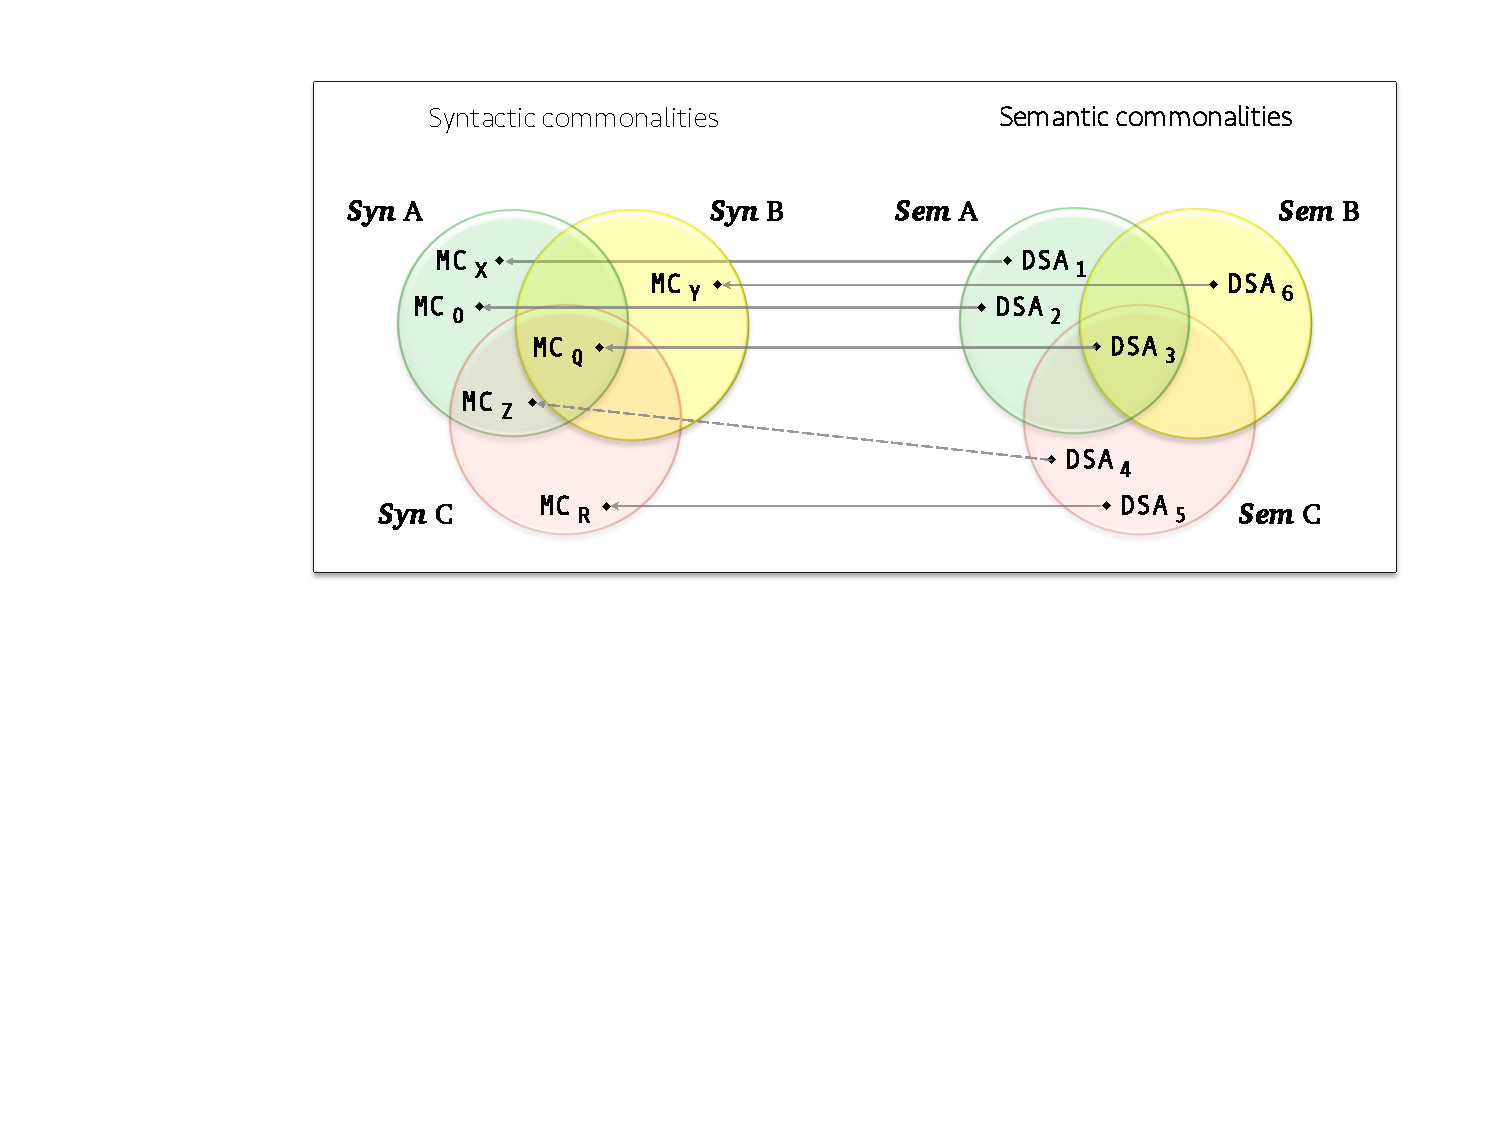
\includegraphics[width=1\linewidth]{images/domains-fig.pdf}
\caption{Commonalities between domains and potential reuse}
\label{fig:domains}
\end{figure}

Commonalities can be found between two ore more DSLs of the input set. That is, we can find metaclasses and domain specific actions that are shared by more than two DSLs. Hence, intersections should be searched among all the possible combinations of the DSLs in the input set. Once those functions are defined and implemented, the second phase is to use them in order to find the intersections among the DSLs of the input set. 

\vspace{-3mm}
\subsubsection{Semantical variability:} Note that the fact that two metaclasses are shared does not imply that all their domain specific actions are the same. In that figure, we see this in the case of MMz. This metaclass is shared by the DSLs A and C but, in each DSL the semantics is different since each of them implement a different DSA for the metaclass. We refer to that phenomenon as \textit{semantical variability}. There are two constructs that share the syntax but that differ in their semantics. In such case, there is potential reuse at the level of the syntax since the metaclass can be defined once and reused in the DSLs but the semantics should be defined differently for each DSLs. 

%there are three DSLs DSLs that are totally independent. That means that they do not share any of their language constructs, and consequently, there is not potential reuse between them. Differently, the two DSLs shown at the right of the figure have overlapping domains. That means that there are a subset of language that are \large\textbf{``equal'' }\normalsize in both DSLs. Note that if two language constructs are the same, we can assume that their specifications are equal and can be reused instead of being replicated.




%Moreover, there are set of DSLs for which the domains can be hierarchically organized \cite[p. 60-61]{voelter:2013}.

%\subsection{Equivalence between language constructs}

%So far, we have based the notion of potential reuse in DSLs on the commonalities existing in a set of DSLs. Nevertheless, this assumption supposes that we are able to compare two language constructs in order to know if they are equivalent. So, now we need to define this \textit{equivalence} relationship. In particular, the comparison of two language constructs relies on two dimensions: (1) comparison of the meta-classes in the abstract syntax; and (2) comparison of the domain-specific actions in the semantics.

